\documentclass{article}

\usepackage[utf8]{inputenc}
\usepackage[T1]{fontenc}    
\usepackage[spanish]{babel} 
\usepackage{fullpage}       
\usepackage{csquotes}
\usepackage[backend=bibtex,style=numeric,sorting=none]{biblatex}
\usepackage{xcolor}
\usepackage{graphicx}
\usepackage{listings}
\usepackage{hyperref}

\usepackage{forest}

\usetikzlibrary{shadows}


\usepackage{float} 
\newcommand{\ile}{\textit{ILE }}
\newcommand{\fig}[1]{\textit{Fig.\ref{fig:#1}}}
\newcommand{\strongitem}[1]{\item \textbf{#1:}}
\newcommand{\imagen}[2]{
  \begin{figure}
  \centering
  \includegraphics[width=0.60\textwidth]{assets/#1}
  \caption{#2}
  \label{fig:#1}
  \end{figure}
}
\newcommand{\centertree}[1]{
  \begin{center}
    \begin{forest}
      blue tree style
      #1
    \end{forest}
  \end{center}
}
\addbibresource{refs.bib}

\title{Desarrollo de un Entorno Integrado de Aprendizaje de Programación
utilizando Editores Proyectivos siguiendo la didáctica de Gobstones}
\date{\today}

\begin{document}


\tikzset{
  blue node style/.style={
    font=\small,
    top color=white,
    bottom color=blue!25,
    rectangle,
    rounded corners,
    minimum size=6mm,
    draw=blue!75,
    very thick,
    drop shadow,
    align=center,
  }
}
\forestset{
  blue tree style/.style={
    for tree={
      parent anchor=south,
      child anchor=north,
      l sep+=5pt,
      blue node style,
      edge={draw=blue!50, thick},
      edge path={
        \noexpand\path [draw, \forestoption{edge}] (!u.parent anchor) -- +(0,-7.5pt) -| (.child anchor)\forestoption{edge label};
      },
      if n children=3{
        for children={
          if n=2{calign with current}{}
        }
      }{},
      delay={if content={}{shape=coordinate}{}}
    }
  }
}


\begin{titlepage}

\newcommand{\HRule}{\rule{\linewidth}{0.5mm}} % Defines a new command for the horizontal lines, change thickness here

\begin{center}

%----------------------------------------------------------------------------------------
%   HEADING SECTIONS
%----------------------------------------------------------------------------------------

% \textsc{\LARGE Propuesta de Trabajo de Inserción Profesional}\\[1.5cm] % Name of your university/college

%----------------------------------------------------------------------------------------
%   TITLE SECTION
%----------------------------------------------------------------------------------------

{ \huge \bfseries Trabajo de Inserción Profesional}\\[0.4cm] % Title of your document

\bigskip
\bigskip
\bigskip
\bigskip
\bigskip
\bigskip
 
\Large \emph{Título:}\\
\textbf{Desarrollo de un Entorno Integrado de Aprendizaje de Programación utilizando Editores Proyectivos siguiendo la didáctica de Gobstones}
\bigskip

\Large \emph{Alumno:}\\
Ariel Alvarez
\bigskip

\Large \emph{Director:}\\
Ing. Nicolás Passerini
\bigskip

\Large \emph{Codirector:}\\
Ing. Javier Fernandes
\bigskip


\Large \emph{Carrera:}\\
Tecnicatura Universitaria en Programación Informática


\bigskip
\bigskip
\bigskip


\includegraphics[width=\textwidth,height=\textheight,keepaspectratio]{assets/logo-unq.jpg}\\[1cm]
\end{center}

\newpage
\tableofcontents


\end{titlepage}

\maketitle

 
\nocite{CuadernoDocenteProgramAR}
\nocite{Maloney_scratch}
\nocite{Gobstones}
\nocite{voelter2014projectional}
\nocite{LanguageModularity}
\nocite{Gamma}
\nocite{TiposGobstones}
\nocite{DowekL11}
\nocite{Inquiry}



\begin{abstract}
Gobstones constituye tanto un lenguaje de programación como secuencia didáctica bien definida que ha demostrado ser eficaz en cursos iniciales universitarios y en escuelas secundarias. En el marco de una comunidad creciente de usuarios, por su uso en cursos universitarios y por la adopción de la secuencia didáctica por parte de los cursos de Program.Ar, se desarrolló una primera versión de un \emph{entorno integrado de aprendizaje de programación} a partir de una implementación de Gobstones sobre un \emph{editor proyectivo}, haciendo uso de sus cualidades intrínsecas para facilitarle al alumno la comunicación de soluciones en términos de conceptos en lugar de trabajar sobre texto crudo, reduciendo así elementos superfluos que pudieran entorpecer la secuencia didáctica.
\end{abstract}



\section{Introducción} \label{intro}

En la República Argentina la enseñanza de la programación en el segundo ciclo primario y primer ciclo secundario se plantea utilizando lenguajes eminentemente visuales \cite{CuadernoDocenteProgramAR}. Esto permite a los alumnos concentrarse en aquello que desean expresar (es decir, el programa que pretenden crear) al eliminar ciertas dificultades inherentes en lenguajes sobre soporte de texto. Por ejemplo, el lenguaje Scratch \footfullcite{scratch}\cite{Maloney_scratch} únicamente permite construcciones \textit{sintácticamente válidas}, ya que cada comando del lenguaje es conformado por bloques visuales encastrables, de tal manera que dos bloques solo encastran cuando constituyen una combinación válida.

Luego, cuando el alumno pasa a un ciclo superior secundario o a la universidad, se le presentan lenguajes basados en texto, en los cuales los errores de sintaxis y de tipado son posibles. En particular en la Universidad Nacional de Quilmes, en la materia de Introducción a la Programación, se utiliza el lenguaje Gobstones \cite{Gobstones}, creado específicamente para la enseñanza de programación.

Si bien Gobstones cuenta con un modelo acotado y una secuencia didáctica clara que lo convierten en una gran herramienta para la enseñanza \footfullcite{gobstonesEsImportante}, al ser basado en texto presenta un nivel de complejidad que puede no resultar adecuado para ciclos inferiores.

En este contexto surgió la propuesta de crear una nueva implementación de Gobstones (acotada en features respecto de la implementación existente hasta el momento) que permitiera únicamente sintaxis válida, de manera similar a los lenguajes visuales ya usados en la enseñanza de la programación, reduciendo así elementos superfluos que pudieran entorpecer la secuencia didáctica planteada para el segundo ciclo de la educación primaria y el primer ciclo de la educación secundaria.
Además se presenta a esta implementación de Gobstones en un entorno que acompañe su secuencia didáctica, tanto desde la construcción de ejercicios y planteo de problemas, como la inclusión incremental de conceptos nuevos durante el proceso de aprendizaje. Se pretende entonces lograr una continuidad entre la enseñanza de la programación utilizando componentes visuales y texto, volviendo más gradual la transición entre uno y otro.

Para lograr una experiencia cercana al texto pero con la ausencia de errores sintácticos, se decidió trabajar sobre un \emph{editor proyectivo}, ya que solamente permite ingresar construcciones sintácticamente válidas en un formato estandarizado (espacios, indentación y demás elementos estéticos son dados por el editor, no por el usuario).

\subsection{Gobstones}

Gobstones constituye un lenguaje y una secuencia didáctica diseñados para la enseñanza de la programación informática, orientada a personas con poca o nula experiencia previa. Propone al programa como una descripción denotacional de un conjunto de ideas que resulta ser ejecutable.
Todo programa Gobstones trabaja sobre un modelo concreto constituído por un tablero de celdas cuadradas, sobre las cuales pueden depositarse o retirarse abalorios de colores utilizando un brazo mecánico que puede moverse por el tablero. El input del programa será un tablero inicial y el output será una transformación sobre ese tablero. De esta manera, el programa aplica una transformación que utiliza primitivas del tablero (poner bolita de color, mover cabezal del brazo mecánico, quitar bolita, etc.) y conceptos fundamentales de programación estructurada como procedimientos, funciones, repeticiones, alternativas condicionales, entre otros.
La secuencia didáctica de Gobstones describe un orden lógico para la presentación de los conceptos fundamentales, comenzando con procedimientos y parametrización, haciendo foco en la necesidad de dividir en subtareas y modularizar. En la \fig{pygobstones_example} puede observarse un ejemplo de programa junto a su tablero resultante.

\imagen{pygobstones_example}{Ejemplo de un programa Gobstones, en el IDE PyGobstones, con su respectivo tablero final}

\subsection{Editores Proyectivos}

El término Editor Proyectivo fue acuñado por Martin Fowler \footfullcite{Fowler} en el año 2005, al intentar plantear un ambiente de desarrollo donde el programador pudiera expresar sus ideas en términos de conceptos en lugar de texto. Lo que vemos como texto pasaría entonces a constituir una representación editable del concepto al que hace referencia (y al cual Fowler llama \textit{representación abstracta}).

Los conceptos del lenguaje son el dominio de los editores proyectivos, y decimos que un programa es una \textit{representación abstracta} construida utilizando dichos conceptos. Para modificar esta representación el programador interactúa con una interfaz de usuario, llamada \textit{representación editable}, sobre la cual la \textit{representación abstracta} se \textit{proyecta} en forma de texto \cite{voelter2014projectional}. En la \fig{projectional-editor} puede observarse un diagrama simplificado de las distintas representaciones de un programa en un editor proyectivo.

\imagen{projectional-editor}{Representaciones de un programa en un editor proyectivo}

A su vez, la \textit{representación abstracta} puede persistirse de diferentes maneras a diferentes soportes, con lo cual se introduce la idea de \textit{representación persistida} para hablar del formato en que guardará el programa, ya sea en una base de datos, un archivo binario, un texto con formato XML, etc.


Algunas consecuencias de los editores proyectivos:
\begin{itemize}
  \item Deja de necesitarse un parser para el lenguaje, volviéndolo más sencillo de extender.
  \item El programador trabaja más cerca de los conceptos que quiere expresar.
  \item Reduce drásticamente los posibles errores de sintaxis.
  \item El editor trabaja directamente con las instancias de los conceptos, con lo cual:
  \begin{itemize}
    \item es más sencillo analizar el programa
    \item se simplifica la construcción de herramientas (ej: refactors, migrado de versiones de lenguaje, intentions, etc)
    \item se mejora la performance del editor al eliminarse la etapa de parseo.
  \end{itemize}
\end{itemize}

\subsection{Organización de este informe}

En la sección \ref{tecnologias} se presenta la tecnología a usar y en la sección \ref{dominio} se describe el desarrollo del modelo conceptual del lenguaje Gobstones en términos de esa tecnología. En la sección \ref{editor} se muestra cómo este modelo conceptual se proyecta sobre el editor. Una vez creado el editor, se procede a implementar el intérprete del lenguaje y la renderización de los tableros inicial y final. Teniendo el lenguaje básico funcionando, se trabaja en la sección \ref{chequeo} sobre el sistema de chequeo de tipos, orientado a asistir al estudiante mediante mensajes de error legibles. En la sección \ref{usabilidad} se analizan problemas típicos de los editores proyectivos y se busca mejorar la experiencia de usuario aplicando diferentes técnicas que facilitan una edición más familiar, es decir, más cercana a una expriencia de edición de texto. Luego en la sección \ref{proyecto} se extiende el proyecto agregando la capacidad de \textit{definir ejercicios}, que constituye un lenguaje específico de dominio cuya finalidad es permitirle al docente plantear ejercicios, desde título y descripción hasta restriciones de features de lenguaje y análisis de código. En la sección \ref{conocimientos} se destacan brevemente los conocimientos aplicados durante el desarrollo del proyecto y por último en la sección \ref{conclusion} se cierra el informe con una conclusión e ideas sobre el camino que el proyecto pudiera seguir a futuro.

\section{Tecnología proyectiva a usar}\label{tecnologias}

De los entornos proyectivos existentes hoy en día, se decidió utilizar el workbench Meta Programming System (MPS) \footfullcite{MPS} \cite{LanguageModularity} de la empresa Jetbrains, en su versión 3.3.
Se trata de un entorno orientado al desarrollo de lenguajes maduro y estable, sobre el cual se realizaron exitosamente diferentes proyectos, entre los cuales se cuentan:
\begin{itemize}
\item MetaR \footfullcite{MetaR}: un IDE que utiliza el lenguaje R para facilitar el análisis de datos biológicos.
\item mbeddr \footfullcite{mbeddr}: un IDE orientado a la programación sobre hardware, que extiende el lenguaje C y soporta verificación formal, máquinas de estado y variabilidad en líneas de productos, entre otros.
\item YouTrack \footfullcite{YouTrack}: un gestor de proyectos.
\end{itemize}

MPS brinda un DSL (lenguaje específico de dominio) para la definición de conceptos puros del lenguaje a implementar, y sobre estos la posibilidad de describir cómo este modelo se renderizará, comportamiento específico para cada concepto, sistema de tipos, etc. Al ser todas estas incumbencias transversales a los conceptos, se organizan en forma de aspectos.
Los conceptos se comportan de manera similar a una clase en programación orientada a objetos, en tanto y en cuanto admiten extensión por herencia e implementación de interfaces. A su vez, estas construcciones determinan las instancias de nodos que compondrán un programa, comparables a los nodos de un árbol de sintaxis abstracta.

A partir de los lenguajes definidos en esta herramienta es posible generar un entorno de desarrollo autónomo o plugins para entornos pre-existentes.

\section{Modelo conceptual del lenguaje Gobstones}\label{dominio}

Se comenzó modelando el lenguaje Gobstones en términos de conceptos. Como puede observarse en el ejemplo de la \fig{ifElse_concept}, para cada concepto pueden definirse sus posibles nodos hijo, propiedades y referencias a otros nodos. Se organizan en una jerarquía, pudiendo extender de otros conceptos e implementar interfaces. En este caso, el concepto \textit{IfElseStatement} extiende del concepto abstracto \textit{Statement}, y sus posibles hijos son una expresión, que será la condición de la alternativa, un bloque de sentencias para el caso en que la condición sea verdadera, y otro bloque de sentencias para el caso contrario.

\imagen{ifElse_concept}{Definición del concepto para la alternativa condicional}

Los conceptos más importantes son \textit{Statement}, que denota un comando, y \textit{Expression} que denota una expresión que puede ser evaluada. De manera simplificada, tenemos que el primer nivel de la jerarquía de sentencias quedó dado por:

\centertree{
  [Statement 
      [Alternative ]
      [Loop]
      [Procedure]
      [Assignment]
  ]
}

\bigskip

\noindent y el primer nivel de la jerarquía de expresiones se compone de:

\centertree{
  [Expression 
      [BinaryOperation]
      [Value]
      [FunctionCall]
  ]
}

\bigskip

Además, se tiene una jerarquía separada para la definición de rutinas:

\centertree{
  [RoutineDeclaration 
    [ProcedureDeclaration] 
    [FunctionDeclaration]
  ]
}


Decimos entonces que un programa Gobstones básico, en el contexto de este editor proyectivo, se encuentra dado por una colección de sentencias y una colección de definición de rutinas, donde el siguiente programa:

\begin{lstlisting}[frame=single] 

program {
  Poner(Rojo)
}

function verdadero(){
  return(True)
}
    
\end{lstlisting}

\noindent corresponde a un modelo conceptual con la estructura:

\centertree{
  [Program 
      [StatementsList
        [NativeProcedure
          [Red]        
        ]
      ]
      [FunctionDeclaration
        [StatementsList
          [Empty]
        ]
        [True]
      ]
  ]
}


\section{Implementación del Editor}\label{editor}

Una vez completado el modelo conceptual con los elementos del lenguaje Gobstones, según la especificación de \textit{Las bases conceptuales de la Programación: Una nueva forma de aprender a programar} \cite{Gobstones}, se procedió a definir el aspecto de editor para cada uno de ellos. Para esto se hace uso de otro DSL provisto por MPS, que permite definir los layouts en los cuales los conceptos se renderizarán.

La finalidad de este editor es proveer una interfaz de usuario que brinde una experiencia similar a la edición de texto, pero permitiendo únicamente construcciones válidas. Para lograr esto, internamente se hace una distinción entre nodos ligados al programa, es decir, nodos que representan conceptos que se escribieron exitosamente y forman parte del programa que se está escribiendo, y nodos en proceso de creación. 
Cuando el usuario comienza a editar un nodo, internamente se crea una instancia de un editor que se encarga de crear el nodo correspondiente a aquello que se está escribiendo, siempre y cuando logre relacionarlo con un concepto válido. De esta manera, funcionalidades como el autocompletado son responsabilidad de la instancia del editor, mientras que otras como los estilos, sugerencias, alertas, etc. son aplicadas sobre las instancias de los nodos de cada concepto.


En la \fig{function_declaration_editor} se observa el aspecto de edición definido para la declaración de funciones. En este quedan relacionadas las propiedades e hijos del concepto \textit{FunctionDeclaration}. Esta definición provee un \textit{binding bidireccional} entre el modelo conceptual y el editor, comparable con un patrón de arquitectura MVP \footfullcite{martinfowler} \footfullcite{microsoftwpf}. Como consecuencia, cualquier cambio en el modelo se verá reflejado instantáneamente en el editor, y cualquier cambio realizado desde el editor modificará los nodos del modelo conceptual; habilitando también la posibilidad de tener diferentes vistas para un mismo modelo, cuya utilidad se verá en la sección siguiente, al lograr dos vistas diferentes para un mismo modelo de tablero.


  \begin{figure}[h]
  \centering
  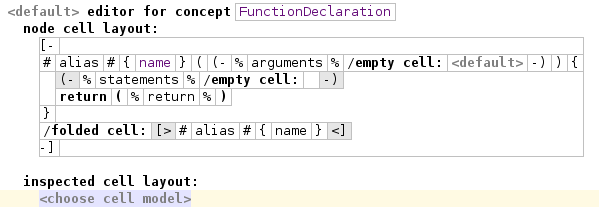
\includegraphics[width=0.80\textwidth]{assets/function_declaration_editor}
  \caption{Definición del aspecto de edición para el concepto de declaración de función}
  \label{fig:function_declaration_editor}
  \end{figure}



El diseño del editor buscó respetar los principios de la programación orientada a objetos. Un claro ejemplo son los subconceptos de \textit{BinaryOperation} tales como los operadores lógicos y aritméticos, que reutilizan una misma vista. Para lograr esto se extrapola el clásico patrón \textit{Template Method} \cite{Gamma}, donde el aspecto de edición del concepto abstracto \textit{BinaryOperation} define el layout de \fig{editor_binary_operation}, y cada subconcepto implementa un alias distinto, correspondiente con el símbolo de su operación.

\imagen{editor_binary_operation}{Definición del aspecto de edición para el concepto abstracto de operación binaria}


\centertree{
  [BinaryOperation
    [{Plus(alias='+')}]
    [{Div(alias='/')}]
    [...]
  ]  
}

Por otro lado, el coloreado de sintaxis, indentación, retorno de carro y demás detalles estéticos se determinan mediante una planilla de estilos, cuidando mantener consistencia entre los diferentes elementos del lenguaje. Por ejemplo, si bien la implementación interna de llamadas a procedimientos nativos y llamadas a procedimientos de usuario son diferentes, ambos comparten los mismos estilos \fig{editor-style}.

  \begin{figure}
  \centering
  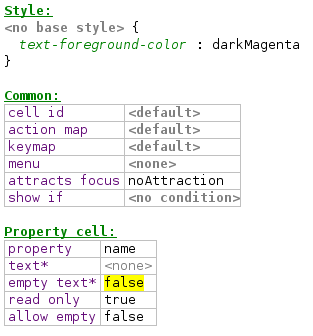
\includegraphics[width=0.40\textwidth]{assets/editor-style}
  \caption{Definición de estilos para la invocación de procedimientos}
  \label{fig:editor-style}
  \end{figure}


Se puede apreciar en \fig{sandbox-editor} que el editor resultante incluye funcionalidades como:
\begin{itemize}
\strongitem{Autocompletado inteligente} solo autocompleta con elementos coherentes con el contexto. En el ejemplo solo autocompleta con sentencias y no expresiones, ya que estas últimas no cumplen propósito alguno en el cuerpo del procedimiento.
\strongitem{Coloreado} Se colorean palabras claves, identificadores, etc. Nótese que los procedimientos y funciones mantienen el mismo color tanto en la declaración como en la invocación, y se diferencian las rutinas nativas de las creadas por el usuario con el uso de negrita en la fuente.
\strongitem{Colapsado de bloques} se pueden colapsar procedimientos y funciones, con el objetivo de facilitar la legibilidad del programa como un todo.
\strongitem{Autoindentación} Las sentencias que se agregan son indentadas automáticamente.
\strongitem{Plantilla de cada herramienta} Al comenzar a escribir una estructura de control, la misma se crea por completo, y permite al usuario rellenar sus partes, proveyendo información sobre qué tipo de elementos corresponden a cada parte. En la imagen, puede notarse esto en la rama falsa de la alternativa condicional.
\end{itemize}

  \begin{figure}
  \centering
  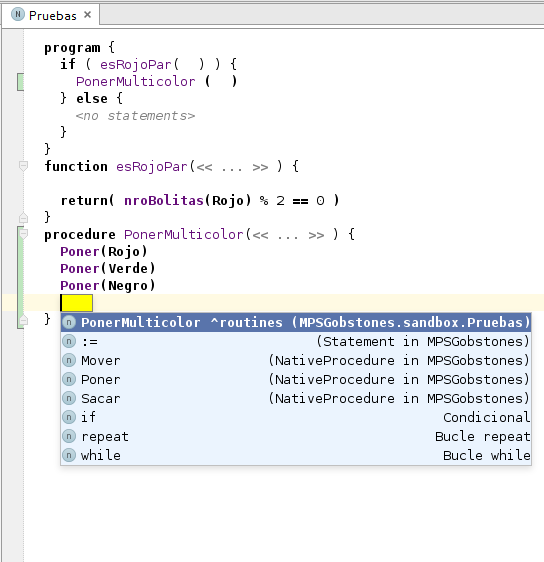
\includegraphics[width=0.45\textwidth]{assets/sandbox-editor}
  \caption{Editor proyectivo de Gobstones}
  \label{fig:sandbox-editor}
  \end{figure}

\section{Implementación del Intérprete}\label{interprete}

Una vez definido el editor proyectivo debemos ser capaces de ejecutar el programa. En esta instancia se presentaron varias alternativas de implementación posibles: compilando o traduciendo a otro lenguaje que luego será ejecutado, es decir, generando de código; o interpretando el programa sin generar código. La generación de código hubiera implicado depender de un compilador o una VM específica, y por consiguiente hubiera complejizado la instalación del producto final (ya sea dependiendo de que la máquina donde se fuera a usar la herramienta final poseyera este compilador, o al verse obligado a empaquetar un compilador o implementación de VM junto con el instalador del entorno), con lo cual se optó por desarrollar un intérprete a partir del ambiente de nodos de conceptos.

En esta etapa se hizo uso del aspecto de comportamiento (\textit{behaviour}), que permitió agregar métodos e inicializaciones a los conceptos, utilizando un DSL con una sintaxis similar a Java. Esto fue así porque al momento de implementar el intérprete, la herramienta no contaba con un aspecto dedicado exclusivamente a la interpretación. Sin embargo, futuras versiones de MPS permitirán extensión mediante la definición de nuevos aspectos por parte del usuario, con lo cual una práctica recomendable será encapsular el comportamiento del intérprete en un aspecto distinto del de \textit{behaviour}, y que podremos llamar \textit{interpreter}.

Se definió en el concepto abstracto \textit{Statement} un método \textit{interpret} que toma como argumento un estado del programa, y retorna otro estado del programa. Por defecto la implementación de \textit{interpret} retorna el estado sin cambiarlo, como se observa en \fig{behavior_statement}. En otras palabras, las sentencias quedaron implementadas un patrón \textit{Composite} \cite{Gamma} en el cual cada sentencia realiza su transformación sobre el estado y delega la interpretación en sentencias hijas de ser necesario. 

\imagen{behavior_statement}{Comportamiento del concepto abstracto Statement}

En la \fig{behavior_ifElse} se puede observar cómo la interpretación de la alternativa condicional está dada por una evaluación de su condición, seguida de la interpretación de alguno de sus bloques según esa condición haya resultado verdadera o falsa. La evaluación de esta condición es posible porque, de manera similar a como se implementa la interpretación para cada sentencia, cada \textit{Expression} entiende el mensaje \textit{reduce}, que toma como argumento un estado del programa y retorna una instancia de \textit{InterpreterValue}, la cual encapsula el valor resultante y contiene información del tipo de este valor. 

\imagen{behavior_ifElse}{Interpretación de la alternativa condicional}


\subsection{Contexto de ejecución}

El estado del programa que es necesario para interpretar sentencias y evaluar expresiones quedó determinado por dos pilas: una pila de tableros (instancias de la clase de dominio \textit{Board}) y una pila de contextos, donde se entiende como contexto al conjunto de variables a las que se pueden acceder en un momento dado.

Al implementar rutinas se siguió la especificación de Gobstones al elegir una evaluación \textit{Call by Value} \cite{DowekL11} de los argumentos, lo cual a su vez permitió mantener una implementación sencilla, evaluando primero los argumentos de las rutinas antes de crear el nuevo contexto. 
Cada vez que se invoca un procedimiento, el contexto que se estaba usando se apila y se crea un nuevo contexto con variables asociadas al resultado de evaluar cada argumento, si los hubiere. 

Cabe aclarar que de haberse requerido una implementación \textit{Call By Name} podría haberse llevarse a cabo inicializando las variables en el nuevo contexto con expresiones asociadas al contexto donde fueron definidas, en lugar de asociarlas a valores puntuales. Es decir, en lugar de tener un \textit{InterpreterValue}, se podría haber creado una \textit{ContextAwareExpression}, que únicamente se evaluaría en caso de ser requerida. La complejidad extra de esta implementación habría radicado en controlar los posibles \textit{memory leaks} que se pudieran generar al mantener referencias a diferentes contextos y guardar el resultado de la primer evaluación para no recalcularlo en evaluaciones posteriores.

Volviendo a la implementación actual, para el caso de las funciones no solo se debe apilar el contexto de variables, sino que también debe clonarse el estado existente del tablero y apilarse, ya que en Gobstones las funciones no realizan efectos de lado, sino que todo efecto aplicado al tablero desaparece una vez que la función retorna un valor. Esto queda claro en \fig{behavior_function_invocation}, donde la invocación de función primero evalúa sus argumentos, crea un \textit{IsolatedContext} con esos argumentos inicializados, y luego evalúa su cuerpo dentro de ese contexto.


  \begin{figure}[h]
  \centering
  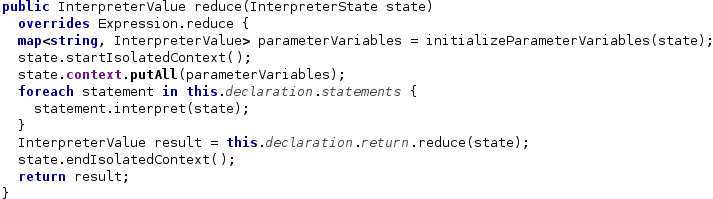
\includegraphics[width=0.75\textwidth]{assets/behavior_function_invocation}
  \caption{Interpretación y cambio de contexto en la invocación de una función}
  \label{fig:behavior_function_invocation}
  \end{figure}
  
\subsection{Clases de dominio de Gobstones}

El proyecto se organiza en varios subproyectos o módulos: un proyecto para el editor, otro para definir el tablero como componente customizado, y otro más para el modelo puro de Gobstones. En este último se definieron las entidades que constituyen el dominio de Gobstones y su comportamiento, tales como el tablero, las celdas, las bolitas, entre otros, utilizando una implementación proyectiva del lenguaje Java. En este modelo quedaron definidas las funcionalidades nativas que le permiten al intérprete interactuar con el tablero de forma tal que, por ejemplo, la interpretación del procedimiento \textit{Poner(<color>)} se termina traduciendo en un mensaje \textit{board.addStones(Color color, int quantity)}. En otras palabras, toda la lógica perteneciente a los elementos concretos de Gobstones queda encapsulada en estas clases de dominio, en su módulo específico e independiente de los otros módulos.
Estas clases constituyen una de las porciones de código más ejecutadas del proyecto y requirieron el uso de estructuras de datos adecuadas para evitar un impacto notable en la performance, no sólo en términos de procesamiento, sino también en generación de instancias. En particular, el tablero guarda la información de sus celdas en un TreeSet \footfullcite{treeSet} para unicamente generar la cantidad de instancias de celdas necesaria. Si bien otras optimizaciones más agresivas eran posibles, no surgió la necesidad de aplicarlas y muchas hubieran implicado reducir la calidad del diseño trabajando sobre estructuras de más bajo nivel.

\subsection{Edición del tablero inicial}

Para editar el tablero inicial que constituye el input del programa Gobstones se creó un editor específico con un \textit{layout table}, como se observa en la \fig{initial_board}. Este tablero se utiliza para inicializar la pila de tableros del estado del programa y puede definirse en un archivo virtual separado de aquel que contiene el código fuente. 

La filosofía detrás de este diseño es que cada componente del programa, desde su tablero inicial y su código hasta su tablero final, son representados como archivos. Esto ayuda a mantener una interfaz de usuario minimalista y una forma de interacción consistente para con los diferentes elementos del entorno.



  \begin{figure}
  \centering
  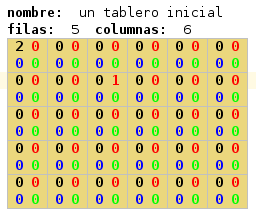
\includegraphics[width=0.34\textwidth]{assets/initial_board}
  \caption{Tablero inicial}
  \label{fig:initial_board}
  \end{figure}


\subsection{Renderización del tablero final}

El tablero final es una vista con \textit{binding unidireccional} que renderiza el estado del tablero que resulta de interpretar el programa Gobstones. Esta vista no fue construida con componentes pre-existentes en MPS, sino que se extendió el editor de MPS creando un componente de Swing\footfullcite{swing} que toma un \textit{Board} y lo renderiza, como se aprecia en la \fig{result_board}. Nótese que tanto el tablero inicial como el tablero final son vistas del modelo \textit{Board}, y se usa una u otra según el tipo de interacción que se desee permitir.


  \begin{figure}
  \centering
  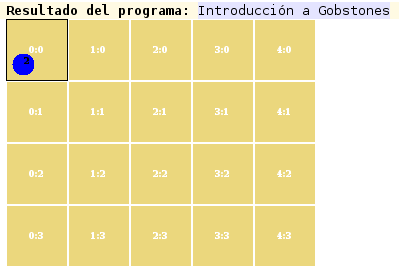
\includegraphics[width=0.34\textwidth]{assets/result_board}
  \caption{Tablero final}
  \label{fig:result_board}
  \end{figure}


\section{Chequeo de tipos}\label{chequeo}

Para implementar el chequeo de tipos se tomó como base el trabajo de inserción profesional de \textit{Federico A. Sawady O’Connor} titulado \textit{Formalización e implementación de un sistema de tipos para el lenguaje de programación Gobstones} \cite{TiposGobstones}, donde se presentan las reglas de inferencia de tipos necesarias para implementar los chequeos de tipos en Gobstones. 
Tomando las reglas puras como base, se implementaron las reglas en MPS dentro del aspecto de sistema de tipos \textit{typesystem}. Por ejemplo, la regla de tipado de las operaciones aritméticas queda denotada por \textit{typeof\_IntegerOperation} en \fig{rule_operation}.
En la \fig{type-check-example} se ejemplifica un error durante el chequeo de tipos, el cual se muestra como un error legible en castellano.

  \begin{figure}
  \centering
  
\includegraphics[width=0.55\textwidth]{assets/rule_operation}
  \caption{Regla de inferencia de tipos para operaciones aritméticas}
  \label{fig:rule_operation}
  \end{figure}
  
\imagen{type-check-example}{Ejemplo de alerta durante el chequeo de tipos}

Además de las reglas de inferencia, es posible crear chequeos manuales por fuera del sistema de tipos. Esto fue de utilidad a la hora de validar que los nombres de procedimientos comiencen con mayúscula y los nombres de funciones con minúscula, ya que al no existir lexers ni parsers, este tipo de restricciones deben declararse en una regla propia.

\section{Mejorando la experiencia de Usuario}\label{usabilidad}

Mantener una experiencia cercana al texto fue uno de los mayores desafíos durante el desarrollo. Por defecto, la edición requiere una escritura en orden prefijo, ya que, por ejemplo, cada operador es padre de sus operandos, y es necesario primero definir la instancia del nodo padre antes de poder determinar sus hijos.
Es decir, al escribir $1+2$ primero es necesario escribir el $+$ y luego se generará la estructura para completar los hijos de izquierda y derecha $\_ + \_$. Sin embargo, esta notación puede resultar incómoda y particularmente antinatural en un curso introductorio a la programación, por lo cual surge la necesidad de permitir una notación infija.

La implementación de notación infija se llevó a cabo declarando acciones de transformación y reemplazo de nodos, para las cuales se declararon sus condiciones disparadoras. 
Volviendo al ejemplo de las operaciones aritméticas (o, en general, de operadores binarios), cuando se comienza escribiendo:

\centertree{
  [1
    [+]
  ]
}



normalmente el editor buscaría reconocer al $+$ como parte de cierto identificador o como posible hijo de $1$, pasando a un estado de error, como se ejemplifica en \fig{aritmetic-operator}

  \begin{figure}[h]
  \centering
  
\includegraphics[width=0.55\textwidth]{assets/aritmetic-operator}
  \caption{Edición de operaciones binarias sin acciones de reemplazo}
  \label{fig:aritmetic-operator}
  \end{figure}
  

Al definir una acción de reemplazo, fue posible identificar esta ocurrencia mediante una expresión regular que reconoce que se escribió un número seguido de un alias de un operador. Luego, se reemplaza la construcción:

\centertree{
  [1
    [+]
    [empty]
  ]
}

\noindent por

\centertree{
  [+
    [1]
    [empty]
  ]
}

\noindent de manera automática y sin que el usuario lo note, mostrándole la edición como en la \fig{aritmetic-operator-action}

  \begin{figure}[h]
  \centering
  
\includegraphics[width=0.45\textwidth]{assets/aritmetic-operator-action}
  \caption{Edición de operaciones binarias con acciones de reemplazo definidas}
  \label{fig:aritmetic-operator-action}
  \end{figure}


Algo similar a lo descripto en el párrafo anterior ocurrió con la alternativa condicional, pero esta vez cuando el usuario intentaba borrar la rama falsa y dejar únicamente la verdadera. Al escribir el \emph{if} se autogeneraba la plantilla correspondiente que se muestra en la \fig{if-statement} pero si se intentaba borrar la rama del \textit{else}, se terminaba borrando toda la construcción del \textit{if}. Esto sucedía porque el borrado se realizaba por nodo, y la alternativa estaba conformada por un único nodo. Para evitar este problema se volvió optativa la rama \textit{false} y se definió una acción que se dispare al intentar borrar un \textit{if}, de tal manera que en lugar de borrarlo se elimine su hijo:

\centertree{
  [IfElseStatement
    [TrueBlock]
    [FalseBlock]
  ]
} 

\noindent por otra construcción que mantiene el mismo hijo \textit{TrueBlock} y el padre, pero se borra el hijo \textit{FalseBlock}:

\centertree{
  [IfElseStatement
    [TrueBlock]
    [empty]
  ]
}


  \begin{figure}[h]
  \centering
  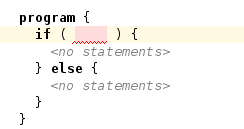
\includegraphics[width=0.40\textwidth]{assets/if-statement}
  \caption{Editor de la alternativa condicional con dos ramas}
  \label{fig:if-statement}
  \end{figure}


\section{Definición de Ejercicios}\label{proyecto}

Hasta el momento, las implementaciones existentes de Gobstones carecían del concepto de proyecto como unidad de organización, y sólo se podía tener un archivo fuente principal y una única biblioteca. Sin embargo, esta única biblioteca comenzó a tener dos usos bien diferenciados por parte de docentes y alumnos: por un lado el alumno quería tener siempre disponible rutinas reutilizables que había hecho para otros ejercicios, y por el otro un docente podía querer brindarle al alumno una biblioteca con funciones y procedimientos ya creados, para trabajar sobre un ejercicio en un nivel de abstracción más alto.
Viendo esta dicotomía, se decidió agregar la idea proyecto bajo el rótulo de \emph{ejercicio}, con la intención de permitir no solo declarar enunciados de ejercicios, sino también de poder proveer al alumno de bibliotecas diseñadas por el docente (si el ejercicio en cuestión lo amerita) separadas de las bibliotecas de alumno.

Estas bibliotecas no constituyen \textit{imports} en el sentido tradicional, dado que no se establecen desde el programa, sino que son dependencias inyectadas por el ejercicio. Esto permite agregar bibliotecas sin modificar el lenguaje Gobstones, y por ende sin aumentar la complejidad del programa creado por el alumno. Por el momento no hay implementada una resolución de posibles conflictos de nombres entre diferentes bibliotecas, quedando a discreción de los usuarios.

Siguiendo la filosofía planteada en este proyecto, la definición del ejercicio también se visualiza como un archivo, orientado a ser legible y con apariencia de documentación, como se observa en la \fig{ejercicio1}

\imagen{ejercicio1}{Definición de un ejercicio simple}

A su vez, dentro de la definición del ejercicio es posible declarar qué herramientas del lenguaje no pueden ser usadas dentro de la resolución del mismo, como muestra la \fig{restricciones-ejercicio}

\imagen{restricciones-ejercicio}{Definición de ejercicio con restricciones}

Internamente, todo concepto del lenguaje que implemente la interfaz \textit{CanBeRestricted} aparecerá en la lista de conceptos cuyo uso puede prohibirse. Esto permite reforzar la introducción gradual de conceptos de programación: al presentarle al alumno un problema que no puede resolver con las herramientas que conoce, se genera la necesidad de indagar por aquello que le está faltando. A este tipo de aprendizaje se lo conoce como \textit{aprendizaje basado en problemas} o \textit{aprendizaje por indagación} \cite{Inquiry}, y constituye uno los pilares fundacionales de la secuencia didáctica de Gobstones.


\section{Conocimientos Aplicados}\label{conocimientos}

El presente trabajo requirió la aplicación numerosos conocimientos técnicos y teóricos, entre los cuales se destacan:

\begin{itemize}
  \strongitem{ Programación orientada a objetos} se aplicó de manera transversal a todo el proyecto, desde el modelo puro y las vistas hasta la implementación de intérprete.
  \strongitem{ Teoría de lenguajes} para el chequeo de tipos y diseño del intérprete.
  \strongitem{ Metaprogramación} todo el proyecto es, en sí mismo, una aplicación de metaprogramación.
  \strongitem{ Construcción de interfaces de usuario} fundametal para el diseño de las vistas, ya que al desaparecer la sintaxis y el texto puro, todo lo que ocupa su lugar es constituído por interfaces de usuario.
\end{itemize}


\section{Conclusión}\label{conclusion}

Se ha logrado finalizar exitosamente una primera versión usable de una implementación del lenguaje Gobstones sobre un editor proyectivo. Los conceptos y tecnologías aplicados permitieron agregar numerosas funcionalidades esperables en un entorno de programación moderno sin grandes dificultades, y por su misma naturaleza requirieron prestar particular atención a ciertos problemas de usabilidad que devienen de la no utilización de texto.
La capacidad de definir ejercicios con sus respectivas especificaciones, tableros, bibliotecas y restricciones constituye un aporte novedoso respecto de las implementaciones pre-existentes. Por este mismo motivo la utilidad de esta funcionalidad, así como también posibles modificaciones futuras, queda aún por ser demostrada y dependerá de la respuesta de los usuarios. Otras funcionalidades, especificadas en \textit{Las bases conceptuales de la Programación} \cite{Gobstones} y presentes en \textit{PyGobstones}\footfullcite{PyGobstones}, como la posibilidad de cambiar vestimentas (estilos e imágenes) a los tableros, han resultado ser sumamente útiles a la secuencia didáctica de Gobstones y se proyecta agregarlas en versiones futuras del producto.
Debido a que actualmente el entorno no se expuso aún a una cantidad suficiente de usuarios y testeo manual, y no posee los estilos gráficos propios de Gobstones, no se considera que esté preparado para ser usado aún en un ambiente productivo. 

\section{Anexo}\label{anexo}

Repositorio del proyecto: \url{https://github.com/uqbar-project/projectional-gobstones}

\section{Agradecimientos}

Mi más sincero agradecimiento a los numerosos docentes y compañeros, muchos de ellos potenciales usuarios, que me brindaron invaluables consejos y opiniones, animándome a continur con un producto que espero podrán disfrutar en un futuro cercano.


\newpage
\printbibliography[nottype=online]

\end{document}
